\documentclass[10pt,oneside]{book}
\usepackage[T1]{fontenc}
\usepackage{isabelle,isabellesym}
\usepackage{graphicx}
\usepackage{listings}
\usepackage{color}

% further packages required for unusual symbols (see also
% isabellesym.sty), use only when needed

%\usepackage{amssymb}
  %for \<leadsto>, \<box>, \<diamond>, \<sqsupset>, \<mho>, \<Join>,
  %\<lhd>, \<lesssim>, \<greatersim>, \<lessapprox>, \<greaterapprox>,
  %\<triangleq>, \<yen>, \<lozenge>

%\usepackage{eurosym}
  %for \<euro>

%\usepackage[only,bigsqcap,bigparallel,fatsemi,interleave,sslash]{stmaryrd}
  %for \<Sqinter>, \<Parallel>, \<Zsemi>, \<Parallel>, \<sslash>

%\usepackage{eufrak}
  %for \<AA> ... \<ZZ>, \<aa> ... \<zz> (also included in amssymb)

%\usepackage{textcomp}
  %for \<onequarter>, \<onehalf>, \<threequarters>, \<degree>, \<cent>,
  %\<currency>

% this should be the last package used
\usepackage{pdfsetup}

% urls in roman style, theory text in math-similar italics
\urlstyle{rm}
\isabellestyle{it}

% for uniform font size
%\renewcommand{\isastyle}{\isastyleminor}

%%% smaller margins, wider text

\addtolength{\oddsidemargin}{-.75in}
\addtolength{\evensidemargin}{-.75in}
\addtolength{\textwidth}{1.5in}

% \addtolength{\topmargin}{-.875in}
% \addtolength{\textheight}{1.75in}

%% ========= Macros ===========

\newcommand{\edcomment}[1]{{\sf \color{red} ({#1})}}

% \newcommand{\edcomment}[1]{{\sf ((#1))}}

\begin{document}

\title{Mechanized Abstract Semantics of AADL \\  as implemented by HAMR}
\author{Stefan Hallerstede and John Hatcliff}
\maketitle

\tableofcontents

% sane default for proof documents
\parindent 0pt\parskip 0.5ex

%% ToDo: Figure out how to get Isabelle to generate the session graph
%% below
%
% \begin{center}
%   \includegraphics[width=\textwidth,height=\textheight,keepaspectratio]{session_graph.pdf}
% \end{center}

\newpage

% generated text of all theories
% \input{session}

\part{Static Model Structure}

\input{Model.tex}

\part{Runtime State and Behavior}

\chapter{Representing AADL Runtime State Information}

\input{VarState.tex}
\input{Queue.tex}
\input{PortState.tex}
\input{ThreadState.tex}
\input{SystemState.tex}

\chapter{AADL Runtime Thread Dispatching Behavior}

\input{DispatchLogic.tex}

\chapter{Thread Application Behavior}

\input{App.tex}

\chapter{System Behavior}

\input{Behavior.tex}

\chapter{Verification Framework}

\input{Properties.tex}

% optional bibliography
%\bibliographystyle{abbrv}
%\bibliography{root}

\part{Libraries}

\chapter{State Reordering}

This chapter describes states as partial maps and defines concepts that permit
reasoning and reordering of sequences of states and state updates.

\input{SetsAndMaps}


\part{Examples}

\chapter{Model Examples}

This chapter includes examples of how the HAMR model-driven
development tool chain translates AADL instance model information into
the types defined in Model.thy.   Along with the model information,
lemmas for model well-formedness are generated, and these are
automatically proved by Isabelle.   This information is derived
directly from and is traceable to the representation of AADL model
information in HAMR-generated code.

\section{Temperature Control Example}

\definecolor{commentcolor}{gray}{0.6}
\definecolor{codebackgroundcolor}{rgb}{0.97,0.99,0.94}
\definecolor{paragraphnumbercolor}{rgb}{0.99,0.60,0.60}
\definecolor{jpcolor}{rgb}{0.2,0.0,0.8}
\definecolor{bacolor}{rgb}{0.0,0.5,0.0}
\definecolor{reconciliationcolor}{rgb}{0.2,0.6,0.2}
\definecolor{notbacolor}{rgb}{0.5,0.0,0.0}

\newcommand{\lstbasicstyle}
  %{\linespread{1.9}\ttfamily\listingsize}
  {\ttfamily\scriptsize}

%define a language for listings
\lstdefinelanguage{bless}
  { morekeywords=[2]{ %AADL keywords
    aadlboolean,aadlinteger,aadlreal,aadlstring,
    abstract,access,and,annex,applies,binding,bus,
    calls,classifier,compute,connections,constant,data,delta,device,
    end,enumeration,event,extends,false,feature,features,flow,
    flows,group,implementation,in,inherit,inverse,is,
    list,memory, mod,mode,modes,none,not,of,or,
    out,package,parameter,path,port,private,process,processor,
    properties,property,prototypes,provides,public, %range,
    reference,
    refined,rem,renames,requires,self,set,sink,source,subcomponents,
    subprogram,system,thread,to,true,type,units,virtual,with,
    stop,abort},
  morekeywords=[1]{ %GUMBO keywords
    assume,case,cases,guarantee,handle,initialize,integration,invariants,inv,modifies,state},
  morekeywords=[1]{ %BLESS keywords
    assert,declare,
    availability,while,forall,exists,that,are,numberof,dispatch,sticky,all,
    aperiodic,sporadic,timed,hybrid,xor,implies,iff,sum,product,
    now,variables,if,fi,skip,invariant,bound,cand,cor,null,timeout,states,
    persistent,shared,transitions,computation,delay,
    initial,complete,final,state,count,fresh,on,
    BLESS,Action,Assertion,pre,post,for,  %subBLESS,
    variant,record,array,do,until,boolean,tops,
    shared,spread,fetchadd,fetchand,fetchor,fetchxor,swap,
    def,integer,natural,rational,real,complex,time,
    Typed,Invariant,Precondition,Postcondition,
%   BLESS_Properties,BLESS_Types,
    otherwise,then,else,elsif,abs,
    updated,frozen,always,never,pause,error,propagations,behavior,
    use,types,events},
  sensitive=true,
  morecomment=[l]{--},
  columns=[r]fixed,
  basicstyle=\lstbasicstyle,
  tabsize=2,
  otherkeywords={
    <, <=, ==, >, >=, &, &&, |, ||, !, ->:, ~>:, ~~>:
    <<,>>,&,??,@,',[,],^,:,+=,\{**,**\},->,
    =>,?,!,+=>,:=,
    *!<,*!>,!<,!>, %-[,]->,
    ~>,(,)
    }
  }

\lstdefinelanguage{slang}
{ morekeywords=[1]{ %SLANG keywords
    Option,None,Some,Unit,
    class,def,return,
    @datatype,@record,@spec,
    Contract,Ensures,Invariant,Modifies,Requires,Res,
  },
  sensitive=true,
  morecomment=[l]{//},
  columns=[r]fixed,
  basicstyle=\lstbasicstyle,
  tabsize=2,
  otherkeywords={
    <, <=, ==, >, >=, &, &&, |, ||, !, ->:, -->:
  }  
}

%\definecolor{commentcolor}{gray}{0.6}
%\definecolor{codebackgroundcolor}{rgb}{0.98,0.99,0.95}

\lstset{language=bless,
%    basicstyle=\tiny,
  keywordstyle={\bfseries\color{blue}},  %BLESS identifiers and symbols
  keywordstyle={[2]\bfseries\color{red}}, %AADL identifiers
  commentstyle={\itshape\color{commentcolor}},  %comments
  frame=tb, %single,
  frameround=tttt,
  backgroundcolor= \color{codebackgroundcolor},
% lineskip=-3pt,
% escapechar=\#,  %use to insert some LaTeX command in the listing
% numbers=left
  }



%LINE NUMBERS  4/18/2010
%turn line numbers on
\newcommand{\turnlinenumberson}
{\lstset{language=bless,
  keywordstyle={\bfseries\color{blue}},  %BLESS identifiers and symbols
  keywordstyle={[2]\bfseries\color{red}}, %AADL identifiers
  commentstyle={\itshape\color{commentcolor}},  %comments
  frame=single,
  frameround=tttt,
  backgroundcolor= \color{codebackgroundcolor},
  lineskip=-1pt,
  numbers=left
  }
} %end of \turnlinenumberson

%turn line numbers off
\newcommand{\turnlinenumbersoff}
{\lstset{language=bless,
  keywordstyle={\bfseries\color{blue}},  %BLESS identifiers and symbols
  keywordstyle={[2]\bfseries\color{red}}, %AADL identifiers
  commentstyle={\itshape\color{commentcolor}},  %comments
  frame=single,
  frameround=tttt,
  backgroundcolor= \color{codebackgroundcolor},
  lineskip=-1pt,
  numbers=none
  }
} %end of \turnlinenumbersoff


\subsection{AADL Model Overview}

\begin{figure*}[htbp]
%  \vspace*{-.2cm}
  \centerline{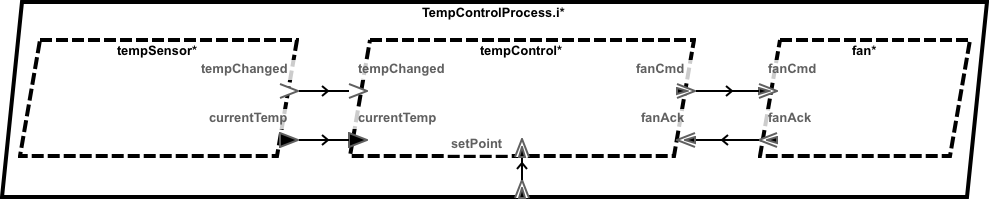
\includegraphics[width=16cm]{temp-control-graphical.png}}
%  \vspace*{-.3cm}
  \caption{Temperature Control Example -- AADL Graphical View}
%  \vspace*{-.3cm}
  \label{fig:temp-control-graphical}
\end{figure*}

Figure~\ref{fig:temp-control-graphical} presents the AADL graphical
view for a simple temperature control system that maintains a
temperature according to a set point containing high and low bounds
for the target temperature.
The periodic \texttt{tempSensor} thread measures the temperature and
transmits the reading on its \texttt{currentTemp} data port.  It sends
a notification on its \texttt{tempChanged} event port if it detects
that the temperature has changed since the last reading.  When the
sporadic (event-driven) \texttt{tempControl} thread receives a
\texttt{tempChanged} event, it reads the value on its
\texttt{currentTemp} data port and compares it with the most recent
set point.  If the current temperature exceeds the high set point or 
drops below the low set point, the fan is turned on or off respectively. 
In turn, the fan acknowledges these commands.
%% sends a \texttt{FanCmd.On} command to cool the temperature.

%% Similar
%% logic will result in \texttt{FanCmd.Off} being sent if the current
%% temperature is below the low set point.  In either case, the
%% \texttt{fan} acknowledges whether it was able to fulfill the command
%% by sending \texttt{FanAck.Ok} or \texttt{FanAck.Error} on its
%% \texttt{fanAck} event data port.

\begin{figure}[htbp]
\begin{lstlisting}[
  language=bless
  ]
thread TempControl
  features
  -- ==== INPUTS ==== 
    currentTemp: in data port TempSensor::Temperature.i;
    tempChanged: in event port;
    fanAck: in event data port CoolingFan::FanAck;
    setPoint: in event data port SetPoint.i;
    -- ==== OUTPUTS ==== 
    fanCmd: out event data port CoolingFan::FanCmd;
  properties
    Dispatch_Protocol => Sporadic;
    Period => 1 sec;
end TempControl    
\end{lstlisting}
\caption{Temperature Control Thread -- AADL Textual View}
\label{fig:temp-control-thread-textual}
\end{figure}

AADL's textual view for the component type definition of the \texttt{TempControl}
thread is shown in Figure~\ref{fig:temp-control-thread-textual}.
Because \texttt{TempControl} is event-triggered, it will be dispatched
by arrival of events on any of the \texttt{tempChanged}, \texttt{fanAck}, 
\texttt{setPoint} ports.  Most interesting for us is the dispatching on the 
arrival of the \texttt{tempChanged} event.  In this case, the 
thread application logic will read the \texttt{currentTemp} data port, 
compare the value to the most recent \texttt{setPoint} values, and
compute an appropriate state for the fan, sending an on/off command
over the \texttt{fanCmd} port if necessary.






\input{TempControlModel}


\chapter{Initial State Examples}

This chapter includes examples of how the HAMR model-driven
development tool chain generates runtime state information into the
Isabelle AADL-HSM state representation.  This information is derived
directly from and is traceable to the representation of AADL model
information and state information in HAMR-generated code.

\section{Temperature Control Example}

\input{TempControlInitialThreadStates}


\end{document}

%%% Local Variables:
%%% mode: latex
%%% TeX-master: t
%%% End:
